% !TeX root = skripta-konstitutivni-vztahy.tex
% !TeX lastmodified = 2018-11-27

\subsection{Chybová funkce (error function)}\label{sec:chybova-funkce}
\begin{itemize}
	\item vychází z~distribuční funkce (CDF),
	\item používá se ve statistice pro predikci chování nějakého vzorku vzhledem ke střední hodnotě souboru.
\end{itemize}

\subsubsection{Vztah CDF a~hustoty pravděpodobnosti}
Funkce hustoty pravděpodobnosti $f_x$ s~mediánem $\mu$ a~směrodatnou odchylkou $\sigma$ je v~relaci s CDF vztahem
\begin{equation}
	F_x(x) = \int\limits_{-\infty}^x f_x(t) \diff t
\end{equation}

\begin{figure}[H]
	\centering
	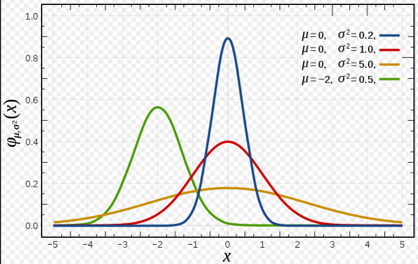
\includegraphics[width=0.7\linewidth]{hustota-pravdepodobnosti}
	\caption{funkce hustoty pravděpodobnosti}
	\label{fig:hustota-pravdepodobnosti}
\end{figure}

\begin{figure}[H]
	\centering
	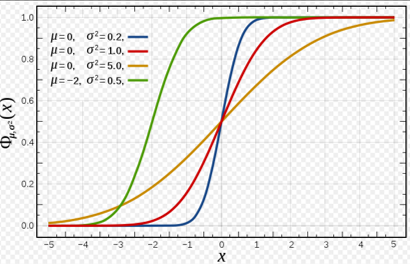
\includegraphics[width=0.7\linewidth]{distribucni-funkce}
	\caption{cumulative distribution function (CDF)}
	\label{fig:distribucni-funkce}
\end{figure}

Chybová funkce vyhodnocená (za podmínky normálního Gaussova rozdělení chyb se směrodatnou odchylkou $\sigma$) pro $\tfrac{x}{\sigma \sqrt{2}}$ udává pro absolutní hodnoty $x$ pravděpodobnost, že měření leží ve vzdálenosti menší než $x$ od střední hodnoty.
\begin{figure}[H]
	\centering
	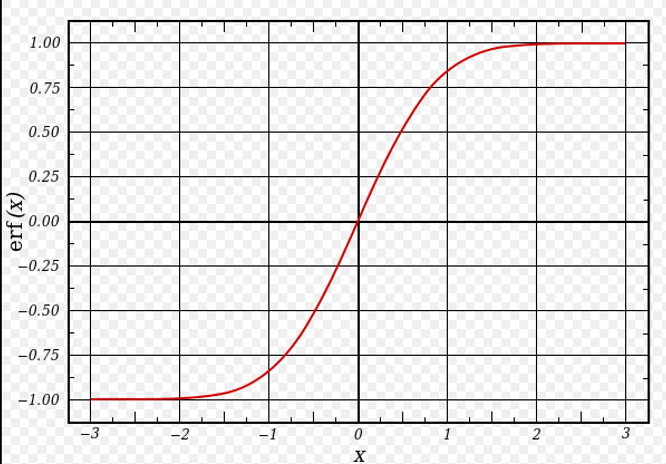
\includegraphics[width=0.7\linewidth]{chybova-funkce}
	\caption{Grafické znázornění chybové funkce}
	\label{fig:chybova-funkce}
\end{figure}

\subsubsection{Matematické vyjádření chybové funkce}
Byla zavedena v~matematice (nazývaná také Gauss error function) je speciální neelementární funkce sigmoidního tvaru, vyskytující se v~pravděpodobnosti, statistice nebo parciálních diferenciálních rovnicích popisujících difuzi.
Je definována takto:
\begin{equation}
	\mathrm{erf}(x) = \frac{2}{\sqrt{\pi}} \int\limits_0^x \exp\left(-t^2\right) \diff t.
\end{equation}

Byla zavedena v~teorii měření (využívající statistiku a~pravděpodobnost) a~název se používá i~při jejím přenosu do jiných oblastí matematiky, které nemají žádný vztah k~charakteristikám chyb měření.

Chybová funkce se vztahuje k~rozdělení měrné energie napjatosti $\varPhi$ (prostřednictvím integrálu normálního rozdělení) rovnicí
\begin{equation}
	\varPhi(x) = \frac{1}{2} + \frac{1}{2} \mathrm{erf}\left(\frac{x}{\sqrt{2}}\right),
\end{equation}
čímž měníme rozsah hodnot z~intervalu $\langle -1;1 \rangle$ na interval $\langle 0;1 \rangle$.
